%%
%% THIS IS FILE: G728DESC.TEX, version of Jan/2008
%% =================================================
%%
%\documentstyle[12pt,epsf,ugst]{book}
\documentclass[12pt]{book}
\usepackage{epsf,ugst}
\usepackage{graphicx}

 
\pagestyle{myheadings}

% Special Parameters 
\evensidemargin           0mm
\oddsidemargin            0mm
\parindent                0mm
\parskip                  2mm
\textheight             250mm %%% 240mm
\textwidth              160mm

%For postscript final deliverable
\topmargin              -20mm
% For PDF final deliverable via PS
%%\topmargin              0mm



% Special font size acronyms used in the first figure
\def\sixsf{\footnotesize\tt}
\def\egtsf{\small\tt}
\def\fivsf{\tiny}
\def\tenrm{\small\tt}
\def\twlsf{\sf}

% Define headers
\def\ugsttitle{ ITU-T Software Tools Library, release 2008: G.728 }
\markboth{ \ugsttitle \hfill Version: \today \hspace{1cm} }{ \hspace{1cm} }

\def\TAU{$\tau_{\alpha,\nu}$}
\def\us{$\mu$s}

%==============================================================================
\begin{document}
%==============================================================================
\SF

\setcounter{chapter}{7}
\setcounter{page}{55}
%=============================================================================
% chapter G.728: The ITU-T 16 kbit/s LD-CELP algorithm 
%=============================================================================

%=============================================================================
% ..... This IS chapter{G.728: LD-CELP etc } .....
%  ... Revision: 
% Mar.1992 - Created (Portuguese)
% Jan.2008 - Translated into English, adapted structure to STL (Simao Campos)
% 
%=============================================================================
\chapter{G.728: The ITU-T low-delay CELP algorithm at 16 kbit/s}
%=============================================================================

Note: The following description is only applicable to the basic G.728
operating mode, 16 kbit/s, both in floating-point (i.e. G.728 main
body \cite{G.728}) and in fixed-point implementation (i.e. G.728 Annex
G \cite{G.728G}). The packet loss concealment for the LD-CELP decoder
(G.728 Annex I \cite{G.728I}) is also described. The other bitrate
extensions (G.728 Annexes H and J) are not part of this description.

CCITT, the predecessor of ITU-T, started an effort in 1985 to define a
successor to then advanced ADPCM coding at 32 kbit/s. Due to the ample
spectrum of its potential applications, extremely demanding
requirements were defined for its performance \cite{Q21-ROs}, which
required quality at least the same as that of G.721 (later superseded
by G.726 operating at 32 kbit/s) for one encoding, and a one-way delay
under 5 ms (but preferably under 2 ms), to avoid the need of echo
cancelers.

The process to identify the performance requirements and objectives
(usually referred to as ``Terms of Reference'', or ToR) for the
16~kbit/s speech coder started in 1985 and lasted until about
1990. The process to identify suitable algorithms and their tests,
after the creation of a group of experts in June 1988, started in
March 1989, with two potential candidates: one from BNR (Canada)
\cite{BNR-coder} and another from AT\&T (USA) \cite{LD-CELP-1}. In
1989, BNR withdrew \cite{BNR-Letter} its candidate, however another
candidate appeared from the Consortium between a company called
VoiceCraft (USA), University of California at Santa Barbara (USA) and
Simon Fraser University (Canada), which would also soon withdraw
\cite{Consort-Letter,LD-VCX-HLD,LD-VCX,LD-VCX2}. This way, AT\&T
continued as the only candidate algorithm proponent in the CCITT
standardization process.

Its algorithm, the LD-CELP {\em (Low-Delay Code-Excited Linear
  Prediction)}, underwent two testing phases (Phase 1 in 1989-1990 and
Phase 2 in 1992) that were organized by volunteers from eight
organizations \cite{Q026}. After tests ensuring that it met all
performance requirements, the LD-CELP algorithm was approved and
published as ITU-T Rec. G.728 \cite{G.728}. Its simplified block
diagram is found in Figure \ref{fig:G728}.

%--------------------------------------------------------------
% FIGURA: Cod+Dec da G.728
%--------------------------------------------------------------
\begin{figure}[hbtp]
  \begin{center}
\setlength{\unitlength}{0.0125in}%

\begin{picture}(450,200)(40,580)
%\put( 85,765){\makebox(0,0)[b]{\raisebox{0pt}[0pt][0pt]{\sixsf INPUT}}}
\put( 85,755){\makebox(0,0)[b]{\raisebox{0pt}[0pt][0pt]{\sixsf PCM}}}
\put(450,760){\makebox(0,0)[b]{\raisebox{0pt}[0pt][0pt]{\sixsf OUTPUT}}}
\put(450,750){\makebox(0,0)[b]{\raisebox{0pt}[0pt][0pt]{\sixsf 16 KBIT/S}}}
\thicklines
\put(340,660){\framebox(70,35){}}
\put(375,685){\makebox(0,0)[b]{\raisebox{0pt}[0pt][0pt]{\sixsf PERCEPTUAL}}}
\put(375,675){\makebox(0,0)[b]{\raisebox{0pt}[0pt][0pt]{\sixsf WEIGHTING}}}
\put(375,665){\makebox(0,0)[b]{\raisebox{0pt}[0pt][0pt]{\sixsf FILTER}}}
\put(430,660){\framebox(40,35){}}
\put(450,680){\makebox(0,0)[b]{\raisebox{0pt}[0pt][0pt]{\sixsf LEAST}}}
\put(450,670){\makebox(0,0)[b]{\raisebox{0pt}[0pt][0pt]{\sixsf ERROR}}}
\put(190,600){\framebox(70,35){}}
\put(225,625){\makebox(0,0)[b]{\raisebox{0pt}[0pt][0pt]{\sixsf SYNTHESIS}}}
\put(225,615){\makebox(0,0)[b]{\raisebox{0pt}[0pt][0pt]{\sixsf FILTER}}}
\put(225,605){\makebox(0,0)[b]{\raisebox{0pt}[0pt][0pt]{\sixsf ADAPTATION}}}
\put(200,660){\framebox(60,35){}}
\put(230,685){\makebox(0,0)[b]{\raisebox{0pt}[0pt][0pt]{\sixsf SYNTHESIS}}}
%\put(230,675){\makebox(0,0)[b]{\raisebox{0pt}[0pt][0pt]{\sixsf }}}
\put(230,665){\makebox(0,0)[b]{\raisebox{0pt}[0pt][0pt]{\sixsf FILTER}}}
\put(105,600){\framebox(60,35){}}
\put(135,625){\makebox(0,0)[b]{\raisebox{0pt}[0pt][0pt]{\sixsf BACKWARD}}}
\put(135,615){\makebox(0,0)[b]{\raisebox{0pt}[0pt][0pt]{\sixsf GAIN}}}
\put(135,605){\makebox(0,0)[b]{\raisebox{0pt}[0pt][0pt]{\sixsf ADAPTATION}}}
\put( 50,660){\framebox(60,40){}}
%\put( 80,690){\makebox(0,0)[b]{\raisebox{0pt}[0pt][0pt]{\sixsf }}}
\put( 80,680){\makebox(0,0)[b]{\raisebox{0pt}[0pt][0pt]{\sixsf EXCITATION}}}
\put( 80,670){\makebox(0,0)[b]{\raisebox{0pt}[0pt][0pt]{\sixsf CODEBOOK}}}
\put(300,680){\circle{20}}
\put(300,685){\line( 0,-1){ 10}}
\put(295,680){\line( 1, 0){ 10}}
\put(260,740){\framebox(80,40){}}
%\put(300,750){\makebox(0,0)[b]{\raisebox{0pt}[0pt][0pt]{\sixsf }}}
\put(300,760){\makebox(0,0)[b]{\raisebox{0pt}[0pt][0pt]{\sixsf BUFFER}}}
\put(300,770){\makebox(0,0)[b]{\raisebox{0pt}[0pt][0pt]{\sixsf SAMPLE}}}
\put(140,740){\framebox(80,40){}}
\put(180,770){\makebox(0,0)[b]{\raisebox{0pt}[0pt][0pt]{\sixsf LOG-PCM}}}
\put(180,760){\makebox(0,0)[b]{\raisebox{0pt}[0pt][0pt]{\sixsf TO LINEAR PCM}}}
\put(180,750){\makebox(0,0)[b]{\raisebox{0pt}[0pt][0pt]{\sixsf CONVERSION}}}
\multiput( 45,590)(9.03846,0.00000){27}{\makebox(0.4444,0.6667){\tenrm .}}
\multiput( 45,715)(9.03846,0.00000){27}{\makebox(0.4444,0.6667){\tenrm .}}
\multiput( 45,590)(0.00000,8.92857){15}{\makebox(0.4444,0.6667){\tenrm .}}
\multiput(280,590)(0.00000,8.92857){15}{\makebox(0.4444,0.6667){\tenrm .}}
\multiput(450,660)(0.00000,-8.42105){10}{\line( 0,-1){  4.211}}
\multiput(450,580)(-7.95699,0.00000){47}{\line(-1, 0){  3.978}}
\multiput( 80,580)(0.00000,8.42105){10}{\line( 0, 1){  4.211}}
\put( 80,660){\vector( 0, 1){0}}
\put(230,635){\vector( 0, 1){ 25}}
\put(450,695){\vector( 0, 1){ 50}}
\put(410,680){\vector( 1, 0){ 20}}
\put(310,680){\vector( 1, 0){ 30}}
\put(275,680){\line( 0,-1){ 60}}
\put(275,620){\vector(-1, 0){ 15}}
\put(135,635){\vector( 0, 1){ 30}}
\put(180,680){\line( 0,-1){ 60}}
\put(180,620){\vector(-1, 0){ 15}}
\put(260,680){\vector( 1, 0){ 30}}
\put(160,680){\vector( 1, 0){ 40}}
\put(110,680){\vector( 1, 0){ 15}}
\put(300,740){\vector( 0,-1){ 50}}
\put(220,760){\vector( 1, 0){ 40}}
\put(110,760){\vector( 1, 0){ 30}}
\put(125,700){\line( 0,-1){ 40}}
\put(125,660){\line( 5, 3){ 34.559}}
\put(160,680){\line(-5, 3){ 34.559}}
\put( 60,705){\makebox(0,0)[lb]{\raisebox{0pt}[0pt][0pt]{\sixsf DECODER REPLICA}}}
\put(290,700){\makebox(0,0)[b]{\raisebox{0pt}[0pt][0pt]{\twlsf --}}}
\put(285,685){\makebox(0,0)[b]{\raisebox{0pt}[0pt][0pt]{\twlsf +}}}
\put(410,705){\makebox(0,0)[b]{\raisebox{0pt}[0pt][0pt]{\sixsf GAIN}}}
\put(410,715){\makebox(0,0)[b]{\raisebox{0pt}[0pt][0pt]{\sixsf CODEVECTOR}}}
\put(410,725){\makebox(0,0)[b]{\raisebox{0pt}[0pt][0pt]{\sixsf OPTIMUM}}}
\put(140,680){\makebox(0,0)[b]{\raisebox{0pt}[0pt][0pt]{\sixsf INDEX}}}
\end{picture}\\*[5mm]

(a) Encoder block diagram \\*[5mm]

\setlength{\unitlength}{0.0125in}%
\begin{picture}(317,145)(40,660)
\thicklines
\put(130,660){\framebox(70,35){}}
\put(165,685){\makebox(0,0)[b]{\raisebox{0pt}[0pt][0pt]{\sixsf SYNTHESIS}}}
\put(165,675){\makebox(0,0)[b]{\raisebox{0pt}[0pt][0pt]{\sixsf FILTER}}}
\put(165,665){\makebox(0,0)[b]{\raisebox{0pt}[0pt][0pt]{\sixsf ADAPTATION}}}
\put(140,720){\framebox(60,35){}}
\put(170,745){\makebox(0,0)[b]{\raisebox{0pt}[0pt][0pt]{\sixsf SYNTHESIS}}}
%\put(170,735){\makebox(0,0)[b]{\raisebox{0pt}[0pt][0pt]{\sixsf SYNTHESIS}}}
\put(170,725){\makebox(0,0)[b]{\raisebox{0pt}[0pt][0pt]{\sixsf FILTER}}}
\put( 45,660){\framebox(60,35){}}
\put( 75,685){\makebox(0,0)[b]{\raisebox{0pt}[0pt][0pt]{\sixsf BACKWARDS}}}
\put( 75,675){\makebox(0,0)[b]{\raisebox{0pt}[0pt][0pt]{\sixsf GAIN}}}
\put( 75,665){\makebox(0,0)[b]{\raisebox{0pt}[0pt][0pt]{\sixsf ADAPTATION}}}
\put( 65,765){\framebox(60,40){}}
%\put( 95,795){\makebox(0,0)[b]{\raisebox{0pt}[0pt][0pt]{\sixsf }}}
\put( 95,785){\makebox(0,0)[b]{\raisebox{0pt}[0pt][0pt]{\sixsf EXCITATION}}}
\put( 95,775){\makebox(0,0)[b]{\raisebox{0pt}[0pt][0pt]{\sixsf CODEBOOK}}}
\put(240,720){\framebox(60,35){}}
\put(270,735){\makebox(0,0)[b]{\raisebox{0pt}[0pt][0pt]{\sixsf \scriptsize POST-FILTER}}}
\put(230,660){\framebox(80,40){}}
\put(270,690){\makebox(0,0)[b]{\raisebox{0pt}[0pt][0pt]{\sixsf CONVERSION}}}
\put(270,680){\makebox(0,0)[b]{\raisebox{0pt}[0pt][0pt]{\sixsf FROM LINEAR}}}
\put(270,670){\makebox(0,0)[b]{\raisebox{0pt}[0pt][0pt]{\sixsf TO LOG-PCM}}}
\put( 65,760){\line( 0,-1){ 40}}
\put( 65,720){\line( 5, 3){ 34.559}}
\put(100,740){\line(-5, 3){ 34.559}}
\put( 80,740){\makebox(0,0)[b]{\raisebox{0pt}[0pt][0pt]{\sixsf GAIN}}}
\put(175,775){\makebox(0,0)[b]{\raisebox{0pt}[0pt][0pt]{\sixsf 16 KBIT/S}}}
\put(175,785){\makebox(0,0)[b]{\raisebox{0pt}[0pt][0pt]{\sixsf PCM}}}
\put(345,670){\makebox(0,0)[b]{\raisebox{0pt}[0pt][0pt]{\sixsf INPUT}}}
\put(345,680){\makebox(0,0)[b]{\raisebox{0pt}[0pt][0pt]{\sixsf OUTPUT}}}
\put(165,695){\vector( 0, 1){ 25}}
\put(220,740){\line( 0,-1){ 60}}
\put(220,680){\vector(-1, 0){ 20}}
\put( 75,695){\vector( 0, 1){ 30}}
\put(120,740){\line( 0,-1){ 60}}
\put(120,680){\vector(-1, 0){ 15}}
\put(200,740){\vector( 1, 0){ 40}}
\put(100,740){\vector( 1, 0){ 40}}
\put(270,720){\vector( 0,-1){ 20}}
\put(310,680){\vector( 1, 0){ 15}}
\put(150,785){\vector(-1, 0){ 25}}
\put( 65,785){\line(-1, 0){ 25}}
\put( 40,785){\line( 0,-1){ 45}}
\put( 40,740){\vector( 1, 0){ 25}}
\end{picture}\\*[5mm]

(b) Decoder block diagram
  \end{center}
  \caption{ Simplified LD-CELP block diagram\label{fig:G728} }
\end{figure}
%--------------------------------------------------------------


%==============================================
\section{General overview}
%==============================================

%--------------------------------------------------
\subsection{General characteristics} 
%--------------------------------------------------

LD-CELP modified the structure present in the classical CELP-type
coders \cite{CELP-original} to meet the performance requirements for
the algorithm, as well as to allow its implementation in
real-time. However, it kept the basic structure of CELP coders, which
is the the search in codebooks using an analysis-by-synthesis approach.

Traditionally, an analog signal is digitized into a 64 kbit/s bitstream
with 8 bits per sample (ITU-T Rec. G.711), hence a 16 kbit/s
bitstream would be equivalent to quantizing using 2 bits per
sample. Since LD-CELP uses a basic frame of five samples, this implies
that the vector quantization codebook has 1024 vectors (represented
by 10-bit indices). Each codevector is the result of a 3-bit scalar
gain and a shape vector of dimension 5 (represented by 7 bits). The
scalar gain has one sign bit and two magnitude bits, being symmetrical
around 0. This allows doubling the range of amplitudes represented by
the shape codebook without duplicating the search complexity for the
optimal codevector.


The codebook was trained with the same perceptual
weighting\footnote{The term {\em perceptual} designates methods that
  explore the way the human hearing treats audio signals.} implemented
in the codec, what takes into account the adaptation effect in the
predictor and of the excitation gain; this has a better performance
than populating the codebook with Gaussian random numbers, which was
the traditional approach for CELP coders \cite{CELP-original}.

After populating the codebook, indices are assigned to these values to
organize the codevectors inside the codebook. To ensure a better SNR
in the decoder for error-prone channels, a pseudo Gray coding was used
for the indices. With this, a single error affecting the codebook
index will shift it to a codeword very close to the original one,
contrary to what would happen if the indices were randomly
distributed.

%--------------------------------------------------
\subsection{Type of algorithm specification}
%--------------------------------------------------

The specification of an algorithm can be made in one of three
methods \cite{LDCELP-VerProc}: bit-exact, bitstream, and algorithm-exact
specification. The bit-exact specification implies that all variables
and operations inside the algorithm have the bit length and
representation precisely defined; this is the type of specification
historically used for ITU speech and audio codecs, e.g. G.722, G.726, and
G.729. Another approach consists in only specifying the bitstream
format (or syntax) and the decoder; additionally, it is common
practice to provide a reference encoder and decoder, which can usually
be modified to reduce complexity or improve performance. This type of
specification was used for regional cellular codec standards in Japan
and USA, e.g. VSELP, for video codecs, as well as in the MPEG suite
of audio and video codecs. Finally, algorithm-exact
specification implies in describing in detail all parts of the
algorithm, without however specifying variable length or precision. An
algorithm specification made in one of these three ways can additionally
be defined in terms of fixed-point arithmetic (only integer variables)
or of floating-point. 

The original G.728 algorithm is specified in terms of floating-point
operations. Therefore, it is a non-bit-exact specification that
describes precisely the operations for its implementation 
\cite{LDCELP-VerProc}. A fixed-point (albeit non-bit-exact)
implementation of G.728 was subsequently designed to enable efficient
implementation in digital circuit multiplication equipment, which
maintained full interoperability with the original floating-point
version\footnote{\sf The concept of interoperability of two
 implementations of an algorithm comes as a consequence of
 algorithm-exact specifications. They refer to the need of two
 different implementations to speak to each other, even though the
 devices are different. For example, a floating-point DSP and a
 fixed-point DSP, or two floating-point DSPs of different
 manufacturers in which number representation has different
 precision. The small operation differences can cause the
 accumulation of errors that, as time goes by, can lead the two
 implementations to diverge, making them fail to interoperate
 \cite{LDCELP-VerProc}.}. An implication of this approach is the need
to define procedures for more sophisticated implementation and
interoperability verification than the ones used for bit-exact
algorithms.

Historically, the choice for an initial implementation in floating-point was only allowed due to the availability at the time of
commercially available floating-point DSPs. Even though they are
common place today, back in early 1990's this was a breakthrough
decision. This was further motivated by the fact that it was uncertain
whether the original time schedule and performance requirements could
be met if the group were to pursue a fixed-point (possibly bit-exact)
implementation. In retrospect, the quality and deadlines targets could
have been met, but the safe approach was to go for a floating-point
specification.


%--------------------------------------------------
\subsection{Delay} 
%--------------------------------------------------

LD-CELP has an algorithmic delay\footnote{\sf The total delay
  introduced by a codec can be defined as the delay intrinsic to the
  encoder, e.g. the number of samples that it needs to buffer {\em
    before} it can start processing samples, plus the time needed by
  the hardware to process the samples or frame. For G.726 ADPCM, the
  algorithmic delay is zero, while the time needed to process the
  sample is non-zero but under 125 \us ; this results in a total delay
  of one sample, or 125 \us. Obviously, the processing time is highly
  dependent on the implementation and cannot be determined {\em a
    priori}.}  of 625 \us ~(five-sample frame) and a (total) one-way
delay of less than 2 ms. To obtain this delay while keeping the
required quality, the designers adopted a backward predictor
adaptation technique.

%--------------------------------------------------
\subsection{Backward adaptation}
%--------------------------------------------------

In the traditional CELP approach, the excitation, the LPC coefficients
and gain are transmitted, while with LD-CELP only the excitation is
transmitted. For this to work, the LPC analysis is made with the
quantized version of the signal and the excitation gain is updated
based on the gain embedded in the samples previously quantized.

In the LD-CELP encoder there are three backward-adaptive structures:
the LPC synthesis filter, the perceptual weighting filter and the
excitation gain unit. In addition to these three structures, the
decoder also has a backward adaptive post-filter.

%========================================================================
% FIGURE: Hibrid windowing
%========================================================================
%Box dimension: 15.10cm x  4.55cm
\begin{figure}[hbtp]
  \begin{center}
    \makebox[ 5.9444in]{
      \vbox to  1.7917in{
        \vfill
        \includegraphics{hybwin}
      }
      \vspace{-\baselineskip}
    }
  \end{center}
  \caption{ LD-CELP hybrid windowing \label{fig:hybwin} }
\end{figure}
%========================================================================


%--------------------------------------------------
\subsection{Windowing used in the adaptation} 
%--------------------------------------------------

In LD-CELP, except for the long-term post-filter in the decoder, all
backward adaptive structures use LPC analysis. The LPC prediction
coefficients are calculated using the auto-correlation method 
\cite{Rabiner-Schafer}. In this method, windowing is necessary to
increase the prediction gain.

Normally, a Hamming window is used, but this is not appropriate for
LD-CELP. The LD-CELP analysis block has only 5 samples, compared to
the conventional 160 to 256 samples normally used. Hence, using a
Hamming window would imply a significant overlap of windows across
frames and a high computational complexity \cite{LD-CELP-FixedPt}. It
was noticed that in the backward adaptation context of LD-CELP, the
Barnwell recursive windowing technique \cite{RecursWind} gave higher
prediction gains than the Hamming windowing, in addition to a higher
subjective quality for the processed speech. For this reason, the
LD-CELP version tested in Phase 1 of subjective assessments used a
modified adaptive windowing \cite{LD-CELP-Phase2,LD-CELP-RecurWind}.
This way, it was possible to obtain a better quality, a more balanced
computational load and a lower complexity for frequent predictor
updates \cite{LD-CELP-Phase1}.

However, aiming at a future fixed-point implementation with minimal
changes compared to the floating-point version (since interoperability
was a requirement), a hybrid windowing technique was developed 
\cite{LD-CELP-FixedPt,G.728}, with results equivalent to those of the
Barnwell version\footnote{\sf The prediction gain loss was below 0.1
  dBm, a very small value.}. This was implemented in the version
tested in Phase 2 of testings and today is present in G.728 (see
Figure \ref{fig:hybwin}). With it, it was possible to keep the same
quality (since the shape of both the hybrid and recursive windows is
the same) while reducing the computational complexity between 20\% and
30\%. The objective was to reduce the complexity by mixing a recursive
portion using the Barnwell technique with a non-recursive one, however
maintaining the overall shape of the Barnwell window.  The windowing
was implemented such that the $m$ most recent samples are superimposed
using the non-recursive portion of the window, and the samples
previous to the $m$-th sample are considering in the recursive portion
of the window. This window has a characteristic that 
non-recursive part has a sinusoidal shape and the recursive part has a
decaying exponential (so as to lessen the influence of older past
samples).

In terms of equations \cite{G.728,LD-CELP-Phase2}, the hybrid window
$w_m(k)$ is defined by:
\[
w_m(k) = \left\{
\begin{array}{ll}
	f_m(k),		&k<m-N\\
	g_m(k), 	&m-N \leq k < m\\
	0,		&k \ge m\\
\end{array} \right.
\]
where
\[
\begin{array}{lll}
	f_m(k) &= & b \alpha^{-[k-(m-N-1)]}\\
	g_m(k) &= & -\sin [c(k-m)]\\
\end{array}
\]
and $0<\alpha<1$, $0<b<1$ and $c$ are constants specific to each of
the backward adaptive structures of the algorithm.

In the auto-correlation method, the i-th auto-correlation coefficient
$R_m(i)$ of the input signal $s(n)$ is calculated as:
\[
R_m(i)
\begin{array}[t]{ll}
	= &\displaystyle\sum_{k=-\infty}^\infty s(k) w_m(k) s(k-i) w_m(k-i)\\
	= &\displaystyle\sum_{k=-\infty}^{m-1} s(k) w_m(k) s(k-i) w_m(k-i)
			\mbox{\ruley{2em}}\\
	= &r_m^{\cal R}(i) + r_m^{\cal N}(i) \mbox{\ruley{2em}}\\
\end{array} 
\]
Where $r_m^{\cal R}(i)$ and $r_m^{\cal N}(i)$ are respectively the
recursive and non-recursive components of the i-th auto-correlation
coefficient described by:
\[
r_m^{\cal R}(i) = \sum_{k=-\infty}^{m-N-1} s(k) s(k-i) f_m(k) f_m(k-i)
\]
and
\[
r_m^{\cal N}(i) = \sum_{k=m-N}^{m-1} s(k) s(k-i) g_m(k) g_m(k-i)
\]

Considering a predictor of order $M$ with an adaptation (update) cycle
of $L$ samples, the i-th auto-correlation coefficient of the next
adaptation cycle will be:
\[
R_{m+L}(i) = r_{m+L}^{\cal R}(i) + r_{m+L}^{\cal N}(i)
\]
with
\[
r_{m+L}^{\cal R}(i) = \alpha^{2L} r_m^{\cal R}(i) + 
         \sum_{k=m-N}^{m+L-N-1} s(k) s(k-i) f_{m+L}(k) f_{m+L}(k-i)
\]
and
\[
r_{m+L}^{\cal N}(i) = \sum_{k=m+L-N}^{m+L-1} s(k) s(k-i) g_{m+L}(k) g_{m+L}(k-i)
\]

Therefore, it can be seen that $r_{m+L}^{\cal R}(i)$ is {\em
recursively} calculated from its value $r_m^{\cal R}(i)$ from the
previous adaptation cycle and that the auto-correlation coefficients
always have a recursive and a non-recursive portion.


%--------------------------------------------------
\subsection{White noise correction} 
%--------------------------------------------------

The use of the auto-correlation method for the calculation of the LPC
coefficients has embedded in it the calculation of the inverse of the
auto-correlation matrix, even though this is not explicitly made in
methods such as the Levinson-Durbin method, where the prediction (and
reflection) coefficients are iteratively calculated.

However, these are equivalent operations, and if the auto-correlation
matrix is ill-conditioned\footnote{\sf The auto-correlation matrix can
  be ill-conditioned because the signal representation has a finite
  numeric precision.}, the LPC coefficients calculated by the
Levinson-Durbin method can lead to an unstable filter. This effect
will be even more pronounced when high-order LPC filters are used, as
in this case.  A simple technique to reduce the matrix
ill-conditioning consists in adding white noise to the signal on which
the prediction will be made, since this will fill the spectral valleys
with noise and would reduce the dynamic range of the spectrum. From
the computational point of view, however, it is interesting to adopt
an equivalent procedure, designated in G.728 as ``white noise
correction''.

Let's consider a voice signal $s(k)$ whose auto-correlation function is $R_s(i),
i=1..M$, where $M$ is the prediction filter order. In a synthetic
notation, 
\[
          s(k) \longleftrightarrow R_s(i)
\]

Similarly, we can associate to a white noise signal $n(k)$ an
auto-correlation function $R_n(i)$, or:
\[
          n(k) \longleftrightarrow R_n(i)
\]

If we add signal and noise, the resulting auto-correlation function $R(i)$ is:
\[
          s(k) + G . n(k) \longleftrightarrow R(i) = R_s(i) + G . R_n(i)
\]

where G is a constant designated white noise correction factor. The
SNR is given as a function of G:
\[
  \mbox{\it SNR}_{dB} = 20 \log_{10} \pmatrix{\Frac{1}{G}\cr}
\]

As $n(k)$ is a white noise, its auto-correlation function is given by:
\[
      R_n(i) = \cases{1, &{\sf if} i=0 \cr
		      0, &{\sf otherwise}\cr
		     }
\]
Consequently:
\[
      R(i) = \cases{ R_s(0)+G, 	&{\sf if} i=0 \cr
		     R_s(i), 	&{\sf otherwise}   \cr
		   }
\]

This way, it can be seen that it is sufficient to add a certain value
$G$ to the coefficient $R_s(0)$ to reduce the ill-conditioning of the
auto-correlation matrix. The value of $G$ is defined by the level of
noise that one wants to ``add'' to the signal.

In LD-CELP, this technique is used to, without increasing the
computational complexity, add noise at approximately 24 dB below the
signal level ($G$=1/256) and lessen ill-condition of the
auto-correlation matrix for the LPC synthesis filter and the
perceptual weighting filter.

%--------------------------------------------------
\subsection{Bandwidth expansion} 
%--------------------------------------------------

A common technique in CELP coders consists in attenuating the formant
peaks through a bandwidth expansion of the LPC spectrum\footnote{\sf
  Narrow bandwidth formants cause a chirping artifact that reduces the
  subjective quality of the signal. On the other hand, bandwidth
  expansion of the LPC synthesis filter can reduce performance with
  voice-band data, requiring therefore a compromise between voice and
  non-voice signals.}:
\[
    a_i = \lambda ^ i \hat{a}_i
\]
where $\hat{a}_i$ is the i-th coefficient calculated by the predictors
and $\lambda$ is a constant that satisfies $\lambda<1$ and
$\lambda\approx 1$.

The effect of the expansion is to move the predictor poles inside the
unity circle. Additionally, the impulse response of the model gets
shorter, reducing the transmission error propagation inside the
adaptation mechanism.


%--------------------------------------------------
\subsection{Input and output formats} 
%--------------------------------------------------

Since LD-CELP is an algorithm also designed for use in the PSTN, the
input and output signal representation follows the ITU-T Rec. G.711
format (either A or $\mu$ law)\footnote{\sf For the implementation
  verification and interoperability purposes (see G.728 Appendix I),
  however, the input signal format must be linear. Therefore, the
  A/$\mu$-law compression and expansion blocks must be bypassed.}.

Since the internal algorithm operations are performed in linear PCM
format, the first block in Figure \ref{fig:G728}(a) consists in the
expansion of the log-PCM samples into linear format; complimentary,
the last block in Figure \ref{fig:G728}(b), after all decoding
processing, does the compression of the linear samples into the
selected log-PCM law.

%======================================================================
\section{Encoder structures}
%======================================================================

In the following, the LD-CELP encoder blocks are
described, as illustrated in Figure \ref{fig:G728}(a). 

%----------------------------------------------
\subsection{LPC synthesis filter} 
%----------------------------------------------

The synthesis filter uses LPC coefficients and has order 50, and
generates the quantized signal from the de-normalized excitation
vector. The reason for such a high order is explained below.

A very common technique used in speech coders, in particular CELP
coders, is the use of long-term prediction, or forward-adaptive pitch
prediction. Conventional LPC prediction is normally based on a small
number of LPC coefficients (usually, 10 to 12 in narrowband speech signal
\cite[pp.419--420]{Rabiner-Schafer}), what does not allow to do a long
term prediction that takes into account the pitch period. The use of
pitch predictors is needed to make whiter the excitation signal
obtained after a conventional LPC analysis, thus better exploring the
signal predictability. However, since LD-CELP only transmits the
excitation information, the pitch prediction would also need to be
backward-adaptive, as done in \cite{BNR-coder,LD-VCX}. This technique,
however, is very sensitive to transmission errors due to the high
filter orders, what makes the errors to propagate over a large number
of samples. The use of artificial re-initializations could solve the
problem, but since the algorithm was required to operate at high bit
error rates, e.g., $\sf 10^{-2}$ equivalent to 160 errors per
second, this would not work for the LD-CELP \cite{LD-CELP-Phase2}.

Together with the error propagation issue, it was noticed that the
improvement introduced by the pitch predictor for female speakers was
much higher than for male speakers\footnote{\sf This is explained by
two factors. First, since a male pitch period is much longer than
for female talkers, the prediction gain is larger for the latter
case. Second, backward-adaptive predictors use the {\em quantized}
error signal as input, instead of the original error signal. The
resulting quantization noise further reduces the correlation within a
pitch period for male voices. Consequently, the prediction gain is
even lower for male speech.}% \cite{ATT-PrivComm:Cox}.}
\cite{LD-CELP-Phase2}.

This way, with the problems of the backward-adaptive pitch predictor
with transmission errors and the larger importance of the pitch
prediction for female speech, it was decided to explore the
predictability of the female speech using a high-order synthesis
filter predictor, so that most of the pitch values for female speaker
would be covered. It was then found empirically that an order of 50
for the LPC synthesis filter produced good results\footnote{\sf
  Additionally, the backward-adaptive LPC predictor of order 50 showed
  to be more resilient to transmission errors than the backward pitch
  predictor.}, replacing the ``low order LPC predictor and pitch
predictor'' traditionally used in CELP coders.


%----------------------------------------------
\subsection{Perceptual weighting filter}
%----------------------------------------------

The general form of the perceptual weighting filter is \cite{Pond-Percep}:
\[
	W(z)= { 1 - Q(z/\gamma_1) \over 1 - Q(z/\gamma_2) }, 
              0 <\gamma_2<\gamma_1\le1.
\]
where:
\[
     Q(z/\gamma_j) = \sum_{i=1}^M \gamma_j^{i} q_i z^{-i}, j=1,2.
\]
and $q_i$ are the quantized LPC coefficients and $M$ is the LPC
predictor order.

Its function is to model the spectral envelope of the error signal, so
that it becomes similar to the spectrum of the input voice signal,
this way masking the distortion which, without this weighting, could
be perceived by the user. By using the weighted error signal to select
the codevector, this codevector will be the one that, on the decoder,
will produce the lowest quantization noise perceived by the user,
increasing in the decoder the subjective quality \cite{Expl-WeigFilt}.

For CELP coders, $(\gamma_1,\gamma_2=(1.0,0.8)$ are normally used. In
LD-CELP Phase 1 and 2, $(\gamma_1,\gamma_2)=(0.9,0.4)$ and
$(\gamma_1,\gamma_2)=(0.9,0.6)$ were used, respectively, what resulted
in a lower perceived noise level. Parameter $\gamma_2$ was changed to
allow the codec to meet the three transcoding requirement, condition
for which the codec had failed the performance requirement in Phase 1 
\cite{LD-CELP:Exp2-Phase1}.

The predictor order $M$ was set here to 10 to avoid
artifacts\footnote{\sf {\em Artifacts} denote here instabilities with
quasi-periodic signals with long duration (more than 2 to 3 seconds),
as happens with artificial voice signals (ITU-T Rec. P.50), some types
of musical passages, e.g. sustained violin sound, or sustained vocalic
sounds, e.g., {\tt/a/}. These instabilities are reproduced as a change
in the sound timbre this reducing the subjective quality.} that appeared with the use of higher order
filters (e.g. 50, as in the synthesis filter). To compensate for the
low order, instead of using a sub-set of the main predictor
coefficients (which in principle could be the same computational
structure), an independent predictor is applied on the input signal
(noting that the main predictor operates on the quantized
samples). This is justified by two facts: since the perceptual
weighting is not necessary on the decoder, nothing obliges the
prediction to be made on the quantized signal; and (more importantly)
the use of the original signal allows the more precise calculation of
the spectral envelope.

%---------------------------------------------------------
\subsection{Search of optimal excitation codevector}
%---------------------------------------------------------

For each sample vector $s(n)$, a search is made to find which of the
1024 codevectors generates the lowest (perceptually weighted) average
quadratic error. The selected codevector has its index transmitted to
the decoder and is fed back to the adaptive part of the encoder (a
replica of the decoder inside the encoder), to be used as excitation
for the synthesis filter. An efficient search algorithm was selected
for the LD-CELP algorithm 
\cite{LD-CELP-Phase1:HQLD,LD-CELP-Phase1:Globecom}, which is described
in detail in the Recommendation \cite{G.728}.


%--------------------------------------------------------
\subsection{Denormalizing quantized excitation} 
%--------------------------------------------------------

To increase coding efficiency, the 1024 codevectors in the codebook
represent typical excitation (obtained by training of this codebook
from a large corpus of speech signals), whose amplitude has been
normalized. Therefore the excitation vector to be used in the
synthesis filter needs to be denormalized, which is done in the
excitation denormalization block. The adaptation mechanism for this
block is described below.


%--------------------------------------------------
\subsection{Adaptation of excitation gain}
%--------------------------------------------------

The optimal index transmitted to the decoder represents the
normalized value of the excitation vector found for the input
signal. Therefore, for the signal reconstruction (both in encoder and
decoder), it is necessary to calculate the excitation gain value to be
used for the denormalization of the excitation gain. This can be done
using a fixed value pre-determined using a long-term statistical
analysis of the possible gain values (similar to the fixed coefficient
predictors and quantizers) of a large corpus of speech
signals. A more optimal approach is to use an adaptive calculation of the
gain. In LD-CELP, the calculation of the gain uses a mixed technique,
which uses a fixed offset of 32 dB for the gain (empirically
obtained), which is associated to a 10-th order LPC predictor using
the auto-correlation method and hybrid windowing. This predictor
adapts the gain around the fixed offset, in order to increase its precision.

The denormalized error signal $e(n)$ can be expressed in terms of the
excitation gain $\sigma(n)$ and the normalized error $y(n)$ by:
\[
      e(n) = \sigma(n) \ y(n)
\]
If $\sigma_y^2(n)$ and $\sigma_e^2(n)$ are respectively the mean
square values of $y(n)$ and $e(n)$, then:
\[
      \log \sigma_e(n) = \log \sigma(n) + \log \sigma_y(n)
\]
We can predict the excitation gain $\sigma(n)$ from the past values of
the denormalized gain $\sigma_e$ using the predictor:
\[
      \log \sigma(n) = \sum_i^P p_i \log \sigma_e(n - i)
\]
Here, the predictor order is $P$=10.

It should be noted that this predictor, when combined with the last
two equations, can be seen as a predictor with $P$ poles and $P$
zeros that uses $\log\sigma_y(n-i)$ as input:
\[
      \log \sigma(n) =   \sum_i^P p_i \log \sigma  (n - i) 
                       + \sum_i^P p_i \log \sigma_y(n - i)
\]

The gain adaptation is backward-adaptive, as in other parts of
LD-CELP. The use of the auto-correlation method for calculating the
coefficients $p_i$ guarantees the stability of the filters above, what
implies a filter response that falls asymptotically to zero. This
limits the propagation of transmission errors, indicating a certain
robustness of this block to transmission errors. This robustness 
brings the poles and zeros closer together, shortens the predictor impulse
response and further limits the propagation of errors within the algorithm.

%--------------------------------------------------------------
\subsection{Adaptation of perceptual adaptation filter} 
%--------------------------------------------------------------

To adapt the coefficients of the perceptual weighting filter the
auto-correlation method is applied over the buffered (unquantized) input
signal using a hybrid window, white-noise correction, and
the Levinson-Durbin algorithm. The LPC coefficients are then
multiplied by the factors $\gamma_1$ and $\gamma_2$, which define the
degree of perceptual weighting.

%--------------------------------------------------
\subsection{Adaptation of LPC synthesis filter}
%--------------------------------------------------

The LPC predictor coefficients for the synthesis filter are adapted
using the quantized input signal. Similar to the perceptual weighting
filter, hybrid windowing, white noise correction and Levinson-Durbin
algorithm are used (albeit with different parameters for the hybrid
window and a larger order of 50 for the LP filter). After calculation
of the LPC coefficients, these pass through the spectral widening and
then are input to the synthesis filter.



%======================================================================
\section{Decoder structures}
%======================================================================

The decoder structure is found in Figure \ref{fig:G728}(b). The blocks
that are identical to ones in the encoder will not be described
again. The few blocks unique to the decoder are described in the
following.

%--------------------------------------------------
\subsection{Post-filter and its adaptation} 
%--------------------------------------------------

A post-filter \cite{PostFilter-Basic} consists of a time-variant
filter put at the output of a decoder with the intention to improve
the subjective signal quality.

Post-filtering, a technique very common in CELP coders, was not used
in the first phase of testing for two reasons. The distortion
introduced by post-filtering accumulates with multiple transcodings
(tandem), what can compromise speech quality\footnote{\sf The main
  distortion generated by post-filtering is the reduction of the
  bandwidth of the spectral peaks. Its accumulation causes severe
  distortion in the decoded speech.}.  Besides that, post-filtering
introduce phase distortions that can make it difficult to decode
properly voice-band data that relies on phase to carry information
(e.g. DPSK) \cite{LD-CELP-1-rev,LD-CELP-Phase1}.

Since the Phase 1 algorithm did not pass the three-tandem connection
condition, it was modified with introduction of post-filtering for
Phase 2. However, the use of traditional post-filtering would imply
unacceptable distortions for the reasons mentioned above. Then instead
of optimizing the post-filter for each transcoding, it was optimized
for three transcodings, thus implying a smaller amount of
post-filtering for each tandem step \cite{LD-CELP-Phase2}. This
allowed the overall distortion added by the post-filtering to remain
within acceptable levels, while the subjective quality for three
transcodings saw a significant improvement (a 26\% increase in the MOS
scores). Even for a single transcoding there was a good improvement in
the subjective quality. During the Phase 2 tests, the change showed to
be a good compromise, increasing the subjective quality while
maintaining a good performance for voice-band data.

The LD-CELP post-filter consists of three blocks: a long-term
post-filter, a short-term post-filter and an automatic gain control (AGC).

The long-term post-filter (also called pitch post-filter), is
basically a comb filter with a fundamental frequency being the
reciprocal of the pitch period. This filter is described by the
following equation:
\[
    H_l(z) = g_l (1 + b z^{-p})
\]
%%%%%
where $p$ is the pitch period obtained by a pitch predictor and $g_l$
and $b$ are coefficients adapted from 240 buffered excitation
samples. In LD-CELP, $p$ varies between 20 and 140 (57 to 400 Hz).

This way, when this post-filtering is applied to the synthesized
signal, the spectrum regions around the multiples of the fundamental
frequency are emphasized. This emphasizes pitch perception, thus
resulting in a higher subjective quality.

The short-term post-filter, on the other hand, is used to reduce the
audible coding noise by emphasizing the peaks and attenuating the
valleys in the input signal spectrum. This is justified by the fact
that perceptually the regions around LPC spectrum peaks, i.e. the
formant regions, are more important than the regions around the
valleys.

The short-term post-filter is implemented as a low-pass filter with
the same number of poles and zeroes which cascades a first-order
high-pass filter. The high-pass filter serves to compensate the
muffling effect of the first low-pass filter. The general form of the
short-term post-filter is given by:
\[
	H_s(z)= { 1 - A(z/\tilde{\gamma}_1) \over 1 - A(z/\tilde{\gamma}_2) } (1 + \mu z^{-1}), 
              \mbox{ with } 0 <\tilde{\gamma}_1 < \tilde{\gamma}_2 \le 1.
\]
where:
\[
\begin{array}{lll}
   A(z/\tilde{\gamma}_j) &= 
    &\displaystyle \sum_{i=1}^M \tilde{\gamma}_j^{i} a_i z^{-i}, \mbox{ for } j=1,2.\\
   \hfill \mu &= &\tilde{\gamma}_3 k_1 \mbox{\ruley{2em}}\\
\end{array}
\]
and $\tilde{\gamma}_1$,$\tilde{\gamma}_2$ and $\tilde{\gamma}_3$ are constants, $a_i$ are the
LPC coefficients, $M$ is the predictor order and $k_1$ is the first
reflection coefficient.

It should be noted that the high-pass filter is implemented with an
adaptive coefficient, the reflection coefficient $k_1$. Therefore, the
filter characteristics might not always be that of a
high-pass. Long-term speech statistics measurements at the time of
development of the algorithm using about 10 minutes of speech showed
that $k_1<0$ for major part of time (around 92\%) (see Figure
\ref{fig:distr-k1}), thus guaranteeing that filter is a high-pass for
the most part of the of the input signals.

%------------------------------------------------------------
%  Figure with k1 histogram
%------------------------------------------------------------
%Box dimension: 10.41cm x  7.27cm
\begin{figure}[hbtp]
  \begin{center}
    \makebox[10.41cm]{
      \rule{0cm}{6.3cm}
      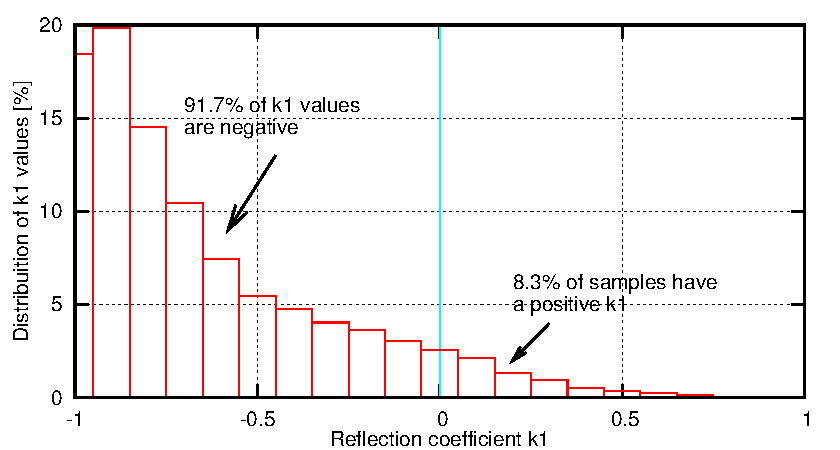
\includegraphics{k1}
    }
  \end{center}
  \caption{Histogram of $k_1$ values for 10 minutes of speech
              \label{fig:distr-k1} }
\end{figure}
%------------------------------------------------------------

In LD-CELP, the filter order of $A(z)$ is 10 and the $a_i$
coefficients, as well as the reflection coefficient $k_1$, are
obtained during the adaptation of the decoder synthesis
filter. Constants $(\tilde{\gamma}_1,\tilde{\gamma}_2,\tilde{\gamma}_3)$ were empirically
determined as (0.65,0.75,0.15).

Finally, the AGC is responsible for making that the power of the
decoded signal after post-filtering be approximately the same as
before post-filtering. The AGC is calculated by the ratio of the
average signal amplitudes before and after post-filtering. This avoids
 too much attenuation or clipping.

%%=============================================================================
%\section{ITU-T STL G.728 Implementation}
%%=============================================================================
%
%{\large\bf This needs to be prepared, similar to other STL chapters. The following has been coarsely adapted from the G.722 chapter.}
%
%This implementation of the G.728 algorithm is composed of several
%source files. The interface routines are in file {\tt g728.c}, with
%prototypes in {\tt g728.h}. The original code of the STL G.728 was
%provided by AT\&T (USA) and its user interface was modified to be
%consistent with the other software modules of the STL.
%
%The problem of storing the state variables was solved by defining a
%structure called ... (was it?).
%
%(describe the state variable structure, if applicable).
%
%The bitstream generated by the STL G.728 encoder has etc...
%
%From the users' perspective, the encoding function is {\tt
%g728\_encode}, and the decoding function is {\tt g728\_decode}.
%Before using these functions, state variables for the encoder and the
%decoder must be initialized respectively by {\tt g728\_reset\_encoder}
%and {\tt g728\_reset\_decoder}. It should be noted that encoder and
%decoder need individual state variables to work properly.
%
%In the following part a summary of calls to the three entry functions
%is found.
%
%{\large\bf From here on, the only change from the G.722 chapter was the substitution of 722 with 728 - hence, a deep review is needed. Kept only for style.}
%
%
%%..........................................................................
%\subsection{{\tt g728\_encode}}
%
%{\bf Syntax: } 
%
%{\tt
%\#include "g728.h"\\
%void g728\_encode (\ttpbox{110mm}{
%            short {\em *inp\_buf}, 
%            short {\em *g728\_frame}, 
%            long  {\em smpno}, 
%            g728\_state {\em *g728\_encode});
%         }
%}
%
%{\bf Prototype: }    g728.h
%
%{\bf Description: }
%
%        Simulation of the ITU-T G.728 64 kbit/s encoder. Takes
%        the linear (16-bit, left-justified) input array 
%        of shorts {\em inp\_buf} (16 bit,
%        right-justified, without sign extension) with {\em smpno}
%        samples, and saves the encoded bit-stream in the array of shorts
%        {\em g728\_frame}.
%
%        The state variables are saved in the structure pointed by {\em
%        g728\_encode}, and the reset can be stablished by making a
%        call to {\tt g728\_reset\_encoder}.
%
%{\bf Variables: }
%\begin{Descr}{\DescrLen}
%\item[\pbox{20mm}{\em inp\_buf}] %\rulex{1mm}\\
%               Is the input samples' buffer with {\em smpno}
%               left-justified 16-bit linear {\tt short} speech samples.
%
%\item[\pbox{20mm}{\em g728\_frame}] %\rulex{1mm}\\
%               Is the encoded samples' buffer; each {\tt short} sample 
%               will contain the encoded parameters as right-justified
%               8-bit samples.
%
%\item[\pbox{20mm}{\em smpno}] %\rulex{1mm}\\
%               Is a long with the number of samples to be encoded from
%               the input buffer {\em inp\_buf}.
%
%\item[\pbox{20mm}{\em g728\_encode}] %\rulex{1mm}\\
%               A pointer to the state variable structure; all the variables 
%               here are for 
%               internal use of the G.728 algorithm, and should not be 
%               changed by the user. Fields of this structure are described 
%               above.
%\end{Descr}
%
%        {\bf Return value: }    
%
%Returns the number of speech samples encoded.
%
%
%%..........................................................................
%\subsection{{\tt g728\_decode}}
%
%{\bf Syntax: } 
%
%{\tt
%\#include "g728.h"\\
%void g728\_decode (\ttpbox{110mm}{
%            short {\em *g728\_frame}, 
%            short {\em *out\_buf}, 
%            int  {\em mode}, 
%            long  {\em smpno}, 
%            g728\_state {\em *g728\_decoder}, );
%         }
%}
%
%{\bf Prototype: }    g728.h
%
%{\bf Description: }
%
%        Simulation of the ITU-T 64 kbit/s G.728 decoder. Reconstructs
%        a linear (16-bit, left-justified) array 
%        of shorts {\em inp\_buf} (16 bit,
%        right-justified, without sign extension) with {\em smpno}
%        samples from the encoded bit-stream in the array of shorts
%        {\em g728\_frame}. 
%
%        The state variables are saved in the structure pointed by {\em
%        g728\_decoder}, and the reset can be stablished by making a
%        call to {\em g728\_reset\_decoder}.
%
%{\bf Variables: }
%\begin{Descr}{\DescrLen}
%\item[\pbox{20mm}{\em g728\_frame}] %\rulex{1mm}\\
%               Is the encoded samples' buffer; each {\tt short} sample 
%               will contain the encoded parameters as right-justified
%               8-bit samples.
%
%\item[\pbox{20mm}{\em out\_buf}] %\rulex{1mm}\\
%               Is the output samples' buffer with {\em smpno}
%               left-justified 16-bit linear {\tt short} speech samples.
%
%\item[\pbox{20mm}{\em mode}] %\rulex{1mm}\\
%               Is an {\tt int} which indicates the operation mode for the
%               G.728 decoder. If equal to 1, the decoder will operate at
%               64 kbit/s. If equal to 2, the decoder will operate at
%               56 kbit/s, discarding the least significant bit of the
%               lower-band ADPCM. If equal to 3, the decoder will
%               discard the two least significant bits of the lower
%               band ADPCM, being equivalent to the 48 kbit/s operation of
%               the G.728 algorithm. It should be noted that, for this
%               implementation of the G.728 algorithm, mode 1-bis is
%               identical to mode 2, and mode 3-bis is identical to mode 3.
%
%\item[\pbox{20mm}{\em smpno}] %\rulex{1mm}\\
%               Is a long with the number of samples in the input
%               encoded sample buffer {\em g728\_frame} to be decoded.
%
%\item[\pbox{20mm}{\em g728\_decoder}] %\rulex{1mm}\\
%               A pointer to the state variable structure; all the variables 
%               here are for 
%               internal use of the G.728 algorithm, and should not be 
%               changed by the user. Fields of this structure are described 
%               above.
%\end{Descr}
%
%        {\bf Return value: }  
%
%Returns the number of speech samples encoded.
%
%
%%..........................................................................
%\subsection{{\tt g728\_reset\_encoder}}
%
%{\bf Syntax: } 
%
%{\tt
%\#include "g728.h"\\
%     void g728\_reset\_encoder (g728\_state {\em *g728\_encoder});
%}
%
%{\bf Prototype: }    g728.h
%
%{\bf Description: }
%
%        Initializes the state variables for the G.728 encoder or decoder.
%        Coder and decoder require each a different state variable.
%
%{\bf Variables: }
%\begin{Descr}{\DescrLen}
%\item[\pbox{20mm}{\em g728\_encoder}] %\rulex{1mm}\\
%        A pointer to the G.728 encoder state variable structure which
%        is to be initialized.
%\end{Descr}
%
%{\bf Return value: }    None.    
%
%
%%..........................................................................
%\subsection{{\tt g728\_reset\_decoder}}
%
%{\bf Syntax: } 
%
%{\tt
%\#include "g728.h"\\
%  void g728\_reset\_decoder (g728\_state {\em *g728\_decoder});
%}
%
%{\bf Prototype: }    g728.h
%
%{\bf Description: }
%
%        Initializes the state variables for the G.728 decoder.
%        Coder and decoder require each a different state variable.
%
%{\bf Variables: }
%\begin{Descr}{\DescrLen}
%\item[\pbox{20mm}{\em g728\_decoder}] %\rulex{1mm}\\
%        A pointer to the G.728 decoder state variable structure which
%        is to be initialized.
%\end{Descr}
%
%
%{\bf Return value: }       None. 
%
%
%%-----------------------------------------------------------------------------
%\section{Portability and compliance}
%
%The portability test for these routines has been done  using the test
%sequences designed by the ITU-T for the G.728 algorithm (available
%from the ITU sales department).  It should be noted that the G.728
%test sequences are not designed to test the QMF filters, but only to
%exercise the upper and lower band encoder and decoder ADPCM
%algorithms. Therefore, testing of the codec with the test sequences
%was done with a special set of test programs that used the core G.728
%upper- and lower-band ADPCM coding and decoding functions. 
%All test sequences were correctly processed.
%
%This module has been tested in VAX/VMS with VAX-C, in the PC
%with Turbo C++ v1.0 (16-bit mode) and GNU-C (32-bit mode), in the Unix
%environment in a Sun workstation with cc, and in HP with 
%gcc.
%
%
%%-----------------------------------------------------------------------------
%\section{Example code}
%
%%..........................................................................
%\subsection {Description of the demonstration programs}
%
%One demonstration program is provided for the G.728 module,
%g728demo.c. In addition, two programs are provided in the distribution
%when compliance testing of the encoder and decoder is necessary,
%tstcg728.c and tstdg728.c\footnote{\SF The demonstration program g728demo.c
%cannot be used for compliance verification because the test vectors
%for G.728 do not foresee processing through the quadrature mirror
%filters.}.
%
%Program {\tt g728demo.c} accepts 16-bit, linear PCM samples sampled at
%16 kHz as encoder input. The decoder also produces files in the same
%format. The bitstream signals out of the encoder are always organized
%in 16-bit, right-justified words that use the lower 8 bits (i.e., 64
%kbit/s). According to the user-specified mode, the decoder will decode
%the G.728-encoded bitstream using 64, 56, or 48 kbit/s (i.e. full 8
%bits, discard 1 bit of the lower band, or discard 2 bits of the lower
%band).
%
%%..........................................................................
%\subsection {Simple example}
%
%The following C code gives an example of G.728 coding and decoding
%using as input wideband speech which is encoded and decoded at either
%64, 56, or 48 kbit/s, according to the user-specified parameter 
%{\em mode}.
%{\tt\small
%\begin{verbatim}
%#include <stdio.h>
%#include "ugstdemo.h"
%#include "g728.h"
%#define BLK_LEN 256
%
%void main(argc, argv)
%  int             argc;
%  char           *argv[];
%{
%  g728_state      encoder_state, decoder_state;
%  int             mode;
%  char            FileIn[180], FileOut[180];
%  short           smpno, tmp_buf[BLK_LEN], inp_buf[BLK_LEN], out_buf[BLK_LEN];
%  FILE           *Fi, *Fo;
%
%  /* Get parameters for processing */
%  GET_PAR_S(1, "_Input File: .................. ", FileIn);
%  GET_PAR_S(2, "_Output File: ................. ", FileOut);
%  GET_PAR_I(3, "_Mode: ........................ ", mode);
%
%  /* Initialize state structures */
%  g728_reset_encoder(&encoder_state);
%  g728_reset_decoder(&decoder_state);
%
%  /* Opening input and output 16-bit linear PCM speech files */
%  Fi = fopen(FileIn, RB);
%  Fo = fopen(FileOut, WB);
%
% /* File processing */
%  while (fread(inp_buf, BLK_LEN, sizeof(short), Fi) == BLK_LEN)
%  {
%    /* Encode input samples in blocks of length BLK_LEN */
%    smpno = g728_encode(inp_buf, tmp_buf, BLK_LEN, &encoder_state);
%
%    /* Decode G.728-coded samples in blocks of length BLK_LEN */
%    smpno = g728_decode(tmp_buf, out_buf, mode, smpno, &decoder_state);
%
%    /* Write 16-bit linear PCM output decoded samples */
%    fwrite(out_buf, smpno, sizeof(short), Fo);
%  }
%
%  /* Close input and output files */
%  fclose(Fi); fclose(Fo);
%}
%\end{verbatim}
%}

%=============================================================================
\section{ITU-T STL G.728 Implementation}
%=============================================================================

This implementation of the G.728 algorithm is composed of source
files in several directories. The floating-point version of the
algorithm can be found in the directory {\tt g728/g728float}. The fixed-point
version is in {\tt g728/g728fixed}.
A third directory, {\tt g728/testvector}, is designed to hold the test
vectors for both versions of the algorithm.
The contents of the testvector directory are not part of the STL, but
can be obtained from G.728 Appendix I on the ITU-T web site.
Similar data structures and interface functions are defined
for both the floating-point and fixed-point G.728 implementations.
The floating-point interface is discussed first.

\subsection {Floating-point G.728}

The source code for the floating-point version of G.728 resides in the
directory {\tt g728/g728float}. All public interface function
declarations and data structures needed to call the coder
can be found in the header file {\tt g728.h}. The package includes a demonstration program, {\tt g728.c},
that shows how to call the encoder, decoder, and decoder with
packet loss concealment. The demonstration program can
run the coder on the G.728 test vectors.

The floating-point version of the coder can be compiled to use either
double precision or single precision floating-point arithmetic. If
compiled with {\tt -DUSEDOUBLES}, g728.h defines the {\tt Float}
typedef as a C {\tt double}. If compiled with {\tt -DUSEFLOATS}, Float
is a C {\tt float}. {\tt Float} is declared in g728.h as: {\tt\small
\begin{verbatim}
#ifdef USEDOUBLES
typedef double Float;
#endif
#ifdef USEFLOATS
typedef float  Float;
#endif
\end{verbatim}
}
Single precision runs faster. Double precision runs slower
but is more likely to give results that are bit-exact across
different machines. When compiling for use with the test vectors
double precision arithmetic should be used.

The include file, g728.h also defines a {\tt Short} type:

{\tt\small
\begin{verbatim}
typedef short  Short;
\end{verbatim}
}

to hold signed 16-bit integers.

\subsection {G.728 Floating-point Encoder}

g728.h defines a C structure, {\tt G728EncData}, to hold the encoder
state variables. Its contents are described in the G.728 standard.
Here we emphasize how to use it, rather than
its internal members. Before calling the encoder
{\tt G728EncData} should be initialized with a call to {\tt g728encinit}:

{\tt\small
\begin{verbatim}
void g728encinit(
     G728EncData *e    /* encoder state, initialize */
);
\end{verbatim}
}

Once initialized, frames of speech can be encoded with:

{\tt\small
\begin{verbatim}
void g728encode(
    Short       *index,  /* output indices */
    Float       *input,  /* input speech */
    int          sz,     /* input size - must be multiple of IDIM */
    G728EncData *e       /* i/o encoder state */	
);
\end{verbatim}
}

The {\tt input} speech should be an array of {\tt Float}s in the range
of -32768. to 32767. {\tt sz} is the dimension of the {\tt input}
array, and must be a multiple of the coder frame size, IDIM.  IDIM is
defined to be 5 in g728.h.  {\tt index} is the output of the
encoder. It is an array of codevector indices that are transmitted to the
decoder.  {\tt index} has dimension sz / IDIM, as one codevector will
be output for each input frame of IDIM speech samples.  Only the least
significant 10 bits of each index value are set.  The 3 bits of gain
index bits are in bits 0 to 2 (0 being the least significant bit), and
the 7 bits of shape index are in bits 3 to 9.  Bits 10 to 15 in each
index value are unused and contain zeros.  If an application desires
to compactly transmit the codevectors for multiple frames, it will
have to extract the lower 10 bits from each index word and pack the
bits.

The floating-point G.728 software package includes utility functions for
converting between {\tt Short}s (16-bit integers) and {\tt Float}s:

{\tt\small
\begin{verbatim}
extern void g728_cpyr2i( /* convert Floats to Shorts,
                          * with saturation and rounding */
    Float *f,   /* input: float array */
    int   sz,   /* input: array size */
    Short *s    /* output: short array */
);
extern void g728_cpyi2r( /* convert Shorts to Floats */
    Short *s,   /* input: short array */
    int   sz,   /* input: array size */
    Float *f    /* output: float array
);
\end{verbatim}
}

These are used by the test program, {\tt g728.c}. A simple encoder loop
that reads in frames of 16-bit linear PCM, encodes them
with floating-point G.728, and outputs the index vectors is in
the following code fragment:

{\tt\small
\begin{verbatim}
#include "g728.h"

Short       ix;         /* output: index */
Short       s[IDIM];    /* input: 16-bit speech */
Float       f[IDIM];    /* converted to Float */
G728EncData e;          /* encode state */

g728encinit(&e);        /* initialize encoder state */
while (fread(s, sizeof(Short), IDIM, speechinf) == IDIM) {
        g728_cpyi2r(s, IDIM, f);        /* convert Short to Float */
        g728encode(&ix, f, IDIM, &e);   /* encode */
        fwrite(&ix, sizeof(Short), 1, indexf);  /* write to file */
}
\end{verbatim}
}

We have omitted the details of opening the files. The code in the {\tt
(mode == M\_ENC)} section of{\tt g728.c} is a more complicated
example that allows frame sizes that are multiples of IDIM, does more
error checking, and also allows byte swapping of the input and output
files.

\subsection {G.728 Floating-point Decoder}

g728.h defines a C structure, {\tt G728DecData}, to hold the decoder
state variables. Many of the decoder state variables replicate
the state variables in the encoder. There are additional
sections for variables associated with the post-filter and
packet loss concealment. As with the encoder, the {\tt G728DecData}
must be initialized before it can be used:

{\tt\small
\begin{verbatim}
void g728decinit(
    G728DecData *d    /* decoder state, initialize */
);
\end{verbatim}
}

Once initialized, frames of speech can be decoded with:

{\tt\small
\begin{verbatim}
void g728decode(
    Float       *speech, /* output: speech */
    Short       *index,  /* input: indices */
    int         sz,      /* input: size - must be multiple of IDIM */
    G728DecData *d       /* i/o: decoder state */	
);
\end{verbatim}
}

{\tt speech} points to the output speech array.  {\tt sz} is the
dimension of the output speech array.  Like at the encoder, it must be a
multiple of the coder frame size, IDIM.  {\tt index} is a pointer to
the array of input codevectors.  As with the encoder {\tt index}
should be dimension sz / IDIM.  Five speech samples will be produced
for each input codevector. The format of the index words is the same
as in the encoder.

If the output speech is to be converted back to 16-bit linear PCM, the
conversion routine should take care of rounding and saturation.
The utility conversion routine, {\tt g728\_cpyr2i}, described above,
takes care of this. Here is a code fragment that can be used
to implement a floating-point decoder:

{\tt\small
\begin{verbatim}
#include "g728.h"

Short       ix;         /* input: index */
Float       f[IDIM];    /* output: speech, Float */
Short       s[IDIM];    /* output: speech, converted to 16-bit int */
G728DecData d;          /* decode state */

g728decinit(&d);        /* initialize decoder state */
while (fread(&ix, sizeof(Short), 1, indexf) == 1) {
    g728decode(f, ix, IDIM, &d);     /* decode */
    g728_cpyr2i(f, IDIM, s);         /* convert to Short */
    fwrite(s, sizeof(Short), IDIM, speechoutf);
}
\end{verbatim}
}

Again we have omitted the details of opening the files.
The code in the {\tt (mode == M\_DEC)} section of {\tt g728.c} is a more
complicated example that allows frame sizes that are multiples of IDIM,
does more error checking, and also allows byte swapping of the input
and output arrays.

An additional interface routine, {\tt g728setpostf}, allows the
post-filter in decoder to be turned on or off. By default, the
post-filter is on after initialization, but it can be disabled as
required by several of the G.728 test vectors:

{\tt\small
\begin{verbatim}
void g728setpostf(
    int          i,     /* in: 1 postfilter on, 0 off */
    G728DecData *d      /* i/o: state variables */
);
\end{verbatim}
}

\subsection {G.728 Floating-point Encoder/Decoder}

The following program fragment shows how to run the encoder and
decoder together. It combines the fragment from the encoder, with the fragment
from the decoder, and uses the utility functions to convert between
Floats and Shorts. The loop sequence is: read in a frame of speech, convert
to Float, encode, decode, convert the output from Float to Short, and write
the resulting speech to a file:

{\tt\small
\begin{verbatim}
#include "g728.h"

Short       ix;         /* index */
Short       s[IDIM];    /* 16-bit speech vector*/
Float       f[IDIM];    /* Float speech vector */
G728EncData e;          /* encode state */
G728DecData d;          /* decode state */

g728encinit(&e);        /* initialize encoder state */
g728decinit(&d);        /* initialize decoder state */
while (fread(s, sizeof(Short), IDIM, speechinf) == IDIM) {
    g728_cpyi2r(s, IDIM, f);       /* convert Short to Float */
    g728encode(&ix, f, IDIM, &e);  /* encode */
    g728decode(f, ix, IDIM, &d);   /* decode */
    g728_cpyr2i(f, IDIM, s);       /* convert to Short */
    fwrite(s, sizeof(Short), IDIM, speechoutf);
}
\end{verbatim}
}

The code that opens and closes the input and output files is omitted.

\subsection {G.728 Floating-point Decoder with Packet Loss Concealment}

The floating-point code supports the Packet Loss Concealment (PLC) algorithm
in G.728 Annex I. This algorithm generates a synthetic
speech output at the decoder and maintains the decoder internal
state variables if the input codevectors are lost in transmission.
This feature is implemented with two more functions. The first PLC function:

{\tt\small
\begin{verbatim}
void g728setfesize(
    int    plc25msec,   /* input: PLC frame size, in 2.5msec */
    G728DecData *d      /* i/o: decoder state */
);	
\end{verbatim}
}

sets the PLC frame size, in increments of 2.5ms (20 samples).  This
function should be called after the G728DecData has been initialized
with a call to g728decinit. If the PLC frame size argument, plc25msec,
is set to 1, each lost frame will correspond to 20 samples. This
variable: plc25msec should be in the range of 1 to 8, corresponding to
a packet loss size of between 2.5 ms (20 samples) and 20 ms (160
samples). If the call to g728setfesize is omitted, the default PLC
frame size is 10~ms (80 samples). The PLC algorithm uses state
variables from the post-filter, so the post-filter must be activated
when running the PLC algorithm.

The second PLC function:

{\tt\small
\begin{verbatim}
void g728decfe(
    Float       *speech,  /* output: speech */
    int         sz,       /* input: size, in samples, PLC framesize */
    G728DecData *d        /* i/o: decoder state */	
);
\end{verbatim}
}

is similar to the g728decode function except it takes no input index vector.
It serves two functions: it signals the decoder that the current frame
is lost, and it generates the synthetic output signal for the frame.
The sz argument is the number of samples in the PLC frame size.
Since there are 20 speech samples in 2.5 ms of speech, the sz argument to
g728decfe should be 20 times the plc25msec argument passed to g728setfesize.
For frames that do not have losses, the standard g728decode function should
be called.

A code fragment that shows how to call the PLC functions for a 10 ms PLC
frame size (80 samples) is shown below:

{\tt\small
\begin{verbatim}
#include "g728.h"

Short       ix[80/IDIM];/* input: index vectors */
Float       f[80];      /* output: Float array */
Short       s[80];      /* output: converted to 16-bit speech */
G728DecData d;          /* decode state */

g728decinit(&d);        /* initialize decoder state */
g728setfesize(4, &d);   /* 4 * 2.5msec frames = 10 msec */
while (fread(ix, sizeof(Short), 80/IDIM, indexf) == 80/IDIM) {
    if (ferasedin())
        g728decfe(f, 80, &d);           /* PLC decode */
    else
        g728decode(f, ix, 80, &d);     /* normal decode */
    g728_cpyr2i(f, 80, s);             /* convert to Short */
    fwrite(s, sizeof(Short), 80, speechoutf);
}
\end{verbatim}
}

As in the previous section, the details on opening the files are
omitted. Function ferasedin() returns 1 if the current frame should
call the packet loss concealment code, and 0 if the standard decoding
routine should be called. The code in the {\tt (mode == M\_PLC)}
section of {\tt g728.c} shows a more complicated version of the PLC loop
that supports setting of the PLC frame size from the command line.

\subsection {Fixed-point G.728}

The source code for the fixed-point version of G.728 resides in the
directory {\tt g728/g728fixed}. All interface functions and data
structures needed to call the coder can be found in the
file {\tt g728fp.h}. The interface mirrors the floating-point
version of the codec, although the routines and data structures
have different names, and the input and output speech arrays are
{\tt Short}s instead of {\tt Float}s.
The fixed-point package also includes a demonstration program, {\tt g728fp.c},
that shows how to call the encoder, decoder, and decoder with
packet loss concealment. The demonstration program can
run the coder on the test vectors. Please note that the fixed-point and
floating-point test vectors are different sets of files.

The fixed-point G.728 algorithm internally uses double precision floating-point
arithmetic to simulate some fixed-point operations. At the time this simulation
was written, this sped up the run-time and allowed the
coder to run in real-time on early Pentium-based computers. With today's
64 bit integer machines and faster processors, there are likely to be
better alternatives for simulating accumulator guard bits.
The fixed-point simulation code should generate bit-exact output for
all the test vectors.

Rather than repeating the interface presented in the floating-point section,
the Table~\ref{tbl:G728-FX-FL} lists the differences between the fixed-point and floating-point versions.

\begin{table}[th]
\Caption{14cm}{\SF Differences between G.728 fixed-point and floating-point versions.
             \label{tbl:G728-FX-FL}}

\begin{center}
\begin{tabular} { | c | c | c | }
 \hline
Object & Floating-Point & Fixed-Point \\ \hline
Include File & g728.h & g728fp.h \\ \hline
Encoder State & G728EncData & G728FpEncData \\ \hline
Decoder State & G728DecData & G728FpDecData \\ \hline
Encoder State Initialize & g728encinit & g728fp\_encinit \\ \hline
Decoder State Initialize & g728decinit & g728fp\_decinit \\ \hline
Encoder & g728encode & g728fp\_encode \\ \hline
Decoder & g728decode & g728fp\_decode \\ \hline
Post-filter Disable & g728setpostf & g728fp\_setpostf \\ \hline
Packet Loss Size & g728setfesize & g728fp\_setfesize \\ \hline
Packet Loss Concealment & g728decfe & g728fp\_eraseframe \\ \hline
\end{tabular}
\end{center}
\end{table}

\subsection {G.728 Fixed-point Encoder/Decoder}

The program fragment below shows how to run the fixed-point encoder and
decoder together. Speech is input from a file, encoded, decoded, and
the output speech is written back to a file:

{\tt\small
\begin{verbatim}
#include "g728fp.h"

Short         ix;       /* index */
Short         s[IDIM];  /* 16-bit speech vector*/
G728FpEncData e;        /* encode state */
G728FpDecData d;        /* decode state */

g728fp_encinit(&e);     /* initialize encoder state */
g728fp_decinit(&d);     /* initialize decoder state */
while (fread(s, sizeof(Short), IDIM, speechinf) == IDIM) {
    g728fp_encode(&ix, s, IDIM, &e);   /* encode */
    g728fp_decode(s, IDIM, &d);        /* decode */
    fwrite(s, sizeof(Short), IDIM, speechoutf);
}
\end{verbatim}
}

This code closely resembles the code fragment for the floating-point code.
Note that the input and output speech arrays to the encoder and decoder
are Shorts so there is no need to call the Float to Short conversion routines.
Input and output speech arrays are 16-bit linear full range PCM.

\subsection {G.728 Demonstration Program}

Both the floating-point and fixed-point versions of the G.728 coder
software provide a demonstration program, defined in {\tt g728.c} and
{\tt g728fp.c}, respectively, that can be used for four
functionalities: encode, decode, decode with packet losses, and encode
and decode a file in a single pass. Scripts are also provided to run
G.728 on the test vectors. The test vectors themselves are not part of
the STL. The floating-point version compiles the program into a binary
called {\tt g728}. The fixed-point version compiles into a binary
called {\tt g728fp}. Since the programs provide an identical user
interface, we will only discuss {\tt g728}. In the examples below,
substitute {\tt g728fp} for {\tt g728} to use the fixed-point version
of the coder.

The demonstration programs expect speech input and output files to be
header-less, and contain binary 16-bit linear full range PCM.  By
default it is assumed that the files are in the native byte order of
the machine. The byte order of the input and output files can be
overridden on the command line with the options {\tt -little} (for
little-endian files) and {\tt -big} (for big-endian files).  When the
-little or -big options are given, the software first determines if
the current machine is a big-endian or little-endian machine.  If the
machine has the same endian characteristics as the requested file, no
byte swapping is performed on the input and output files. If there is
a mismatch, byte swapping is performed. For example, the G.728 test
vector files are little endian files. Giving the -little option on Sun
SPARC and MIPS processors (big-endian machines) will cause the input
files to be byte swapped before processing, and output data streams to
be byte-swapped before being written to files. On Intel processors,
the -little option is a ``no-op''.

Bit-streams are in the format of the ITU G.728 test vectors. For every 5 input
speech samples, a single 16-bit binary word is output. Only the least
significant 10 bits of each 16-bit output word are used.
The G.728 gain index (3 bits) resides in bits 0 to 2 (0 being the least
significant bit), and the shape index (7 bits) resides in bits 3 to 9.

Input PLC mask files are ASCII files that contain '0's and '1's.
A '1' implies the current frame is lost and should be concealed.
A '0' implies the normal decoding routine should be called for the current
frame. The PLC files may also contain newlines and return
characters that will be ignored. If any other character occurs in the file,
it is an error, and the program will exit with an error message.
If the PLC mask file reaches the end of the file
but there are still frames to decode, the PLC file will roll over and
seek back to the beginning of the file. For example, a PLC mask file containing
'00000000000000000001' can be used to introduce a 5\% uniform loss pattern.

The demonstration program supports several other options. Options
should appear in the command line before the mode of the coder:

{\tt -nopostf}\\*
Turn off the post-filter in the decoder. This is required to run many of
the test vectors. For normal operation the post-filter should be on.

{\tt -stats}\\*
PLC concealment option to print out statistics on how
many frames were processed and concealed.

{\tt -plcsize msec}\\*
set the PLC concealment frame size, in milliseconds. This is how much speech
will be concealed by a single lost packet. Only a limited set of values
are acceptable: 2.5, 5, 7.5, 10, 12.5, 15, 17.5 and 20. The default value
is 10 ms.

\subsection {G.728 Demonstration Program Modes}

The program has 4 modes: encode, decode, decode with PLC, and encode and decode.
To run the encoder use:
{\tt\small
\begin{verbatim}
  g728 enc speech.infile bitstream.outfile
\end{verbatim}
}

To run the decoder use:
{\tt\small
\begin{verbatim}
  g728 dec bitstream.infile speech.outfile
\end{verbatim}
}

To run the combined encoder and decoder use:
{\tt\small
\begin{verbatim}
  g728 encdec speech.infile bitstream.outfile speech.outfile
\end{verbatim}
}
To run the decoder with Packet Loss Concealment with the default 10ms
PLC frame size:
{\tt\small
\begin{verbatim}
  g728 plc bitstream.infile plcmask.infile speech.outfile
\end{verbatim}
}

\subsection {G.728 Demonstration Program with Test Vectors}

Scripts ({\tt testall.sh} for Linux and Unix; {\tt testall.bat} for
Windows machines)
are provided for running the demonstration programs on the the G.728 test vectors. The scripts use binary compare functions to see if
the encoder and decoder output files differ
from the expected results.
For the fixed-point code an exact match is expected.
For the floating-point code an exact match is not guaranteed.
However, when compiled to use double-precision
arithmetic ({\tt -DUSEDOUBLES}) we have observed an exact match on
all platforms we have tested the code on.
If the floating-point code is compiled with the option {\tt -DUSEFLOATS},
differences in the test vectors should be expected.
For further details on the test vector verification
procedure when the outputs do not match, please refer to G.278
Appendix I.

A script ({\tt testplc.sh}, {\tt testplc.bat}) is also provided to run
the PLC algorithm on one of the test vectors. This program is only to
demonstrate how to invoke the PLC algorithm, and does not compare the
output with file. It is not possible to compare the outputs to a fixed
file since the PLC algorithm uses a random number generator to extract
the excitation when it determines whether a lost packet frame is in an
unvoiced region of speech. Depending on where the packet losses occur,
the output may be different for each run on the same file.


\bibliographystyle{unsrt}
\bibliography{ugst} %/ default extension is ".BIB" %/

\end{document}
